%!TEX root=RKWard_paper.tex
\section{Fundamentals of the plugin framework}
\label{sec:technical}
In this section we will give a brief overview of the design aspects of \pkg{RKWard}'s plugin framework, 
since this is central to the extensibility of
\pkg{RKWard}. Further details can be found in the annex accompining this paper.

\subsection{Plugin infrastructure}
\label{sec:technical_plugins}
One of the earliest features of \pkg{RKWard} was the extensibility by plugins.
Basically, plugins in \pkg{RKWard} provide complete GUI dialogs, or re-usable
GUI components, which accept user settings and translate those user settings
into \proglang{R} code\footnote{
    Plugins are also used in some other contexts within \pkg{RKWard}, for instance, the
    integrated text editor (\pkg{kate} part) supports extensions via plugins and user scripts. At this point we
    will focus only on plugins generating \proglang{R} code.
}. Thus, the plugin framework is basically a tool set used to define
GUIs for the automatic generation of \proglang{R} code.

Much of the functionality in \pkg{RKWard} is currently implemented as plugins. For example, importing different file
formats relying on the \pkg{foreign} package is achieved by this approach. Similarly,
\pkg{RKWard} provides a modest GUI driven tool set for statistical analysis,
especially for item response theory, distributions, and descriptive
statistical analysis.

\subsubsection{Defining a plugin}
\label{sec:technical_plugins_defining}
Plugins consist of four parts as visualized in Figure~\ref{fig:plugin_structure} 
\citep[see Section~\ref{sec:example_plugin} for an example; for a complete
manual, see][]{Friedrichsmeier2010}:

\begin{figure}[t!]
 \centering
 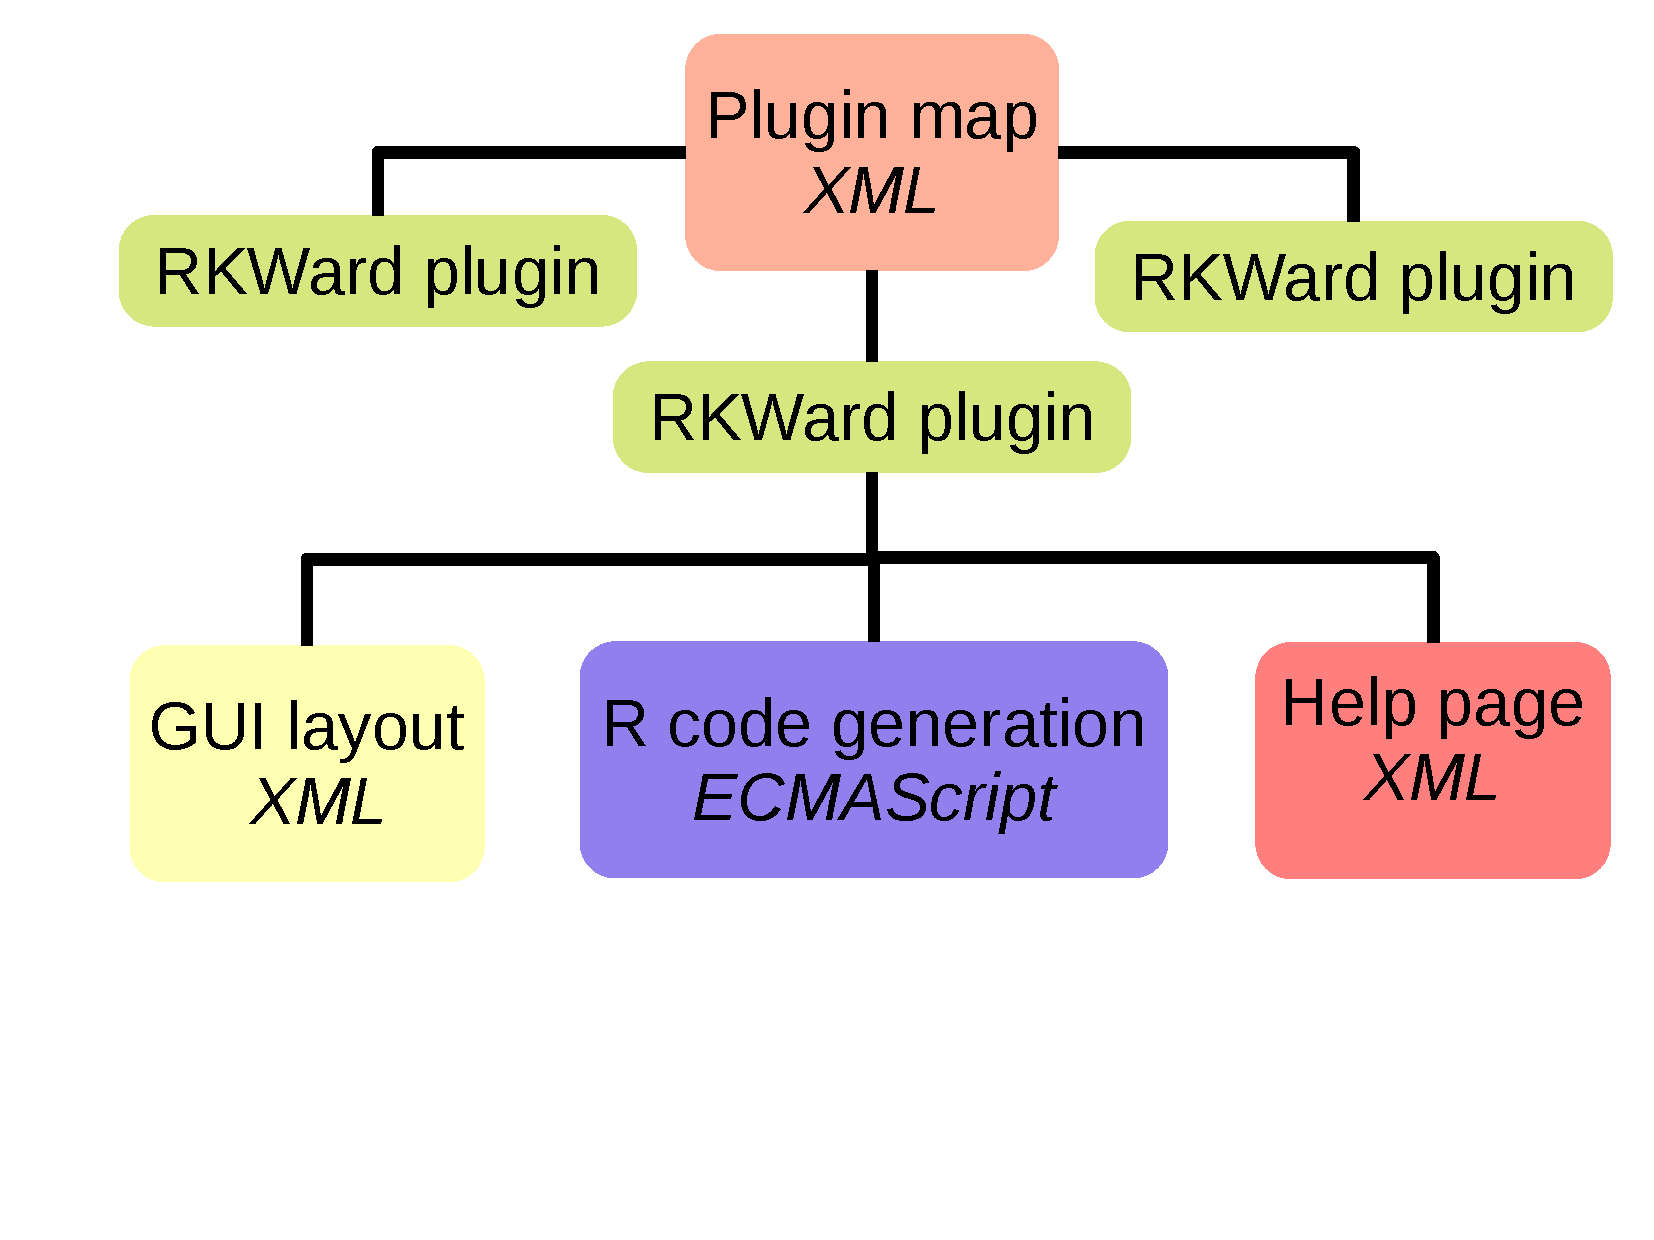
\includegraphics[clip=true,trim=0cm 6cm 0cm 0cm,width=8cm]{./figures/plugin_structure.pdf}
 \caption{Plugin structure of \pkg{RKWard}. One or more plugins are declared in a ``plugin map''. Each plugin is defined by
 two XML files, and one \proglang{ECMAScript} file.}
 \label{fig:plugin_structure}
\end{figure}

\begin{itemize}
    \item
    An XML file (Section~\ref{sec:defining_menu_hierarchy}), 
    called a ``plugin map'', is used to declare one or more plugins, each
    with a unique identifier. For most plugins, the plugin map also defines the
    placement in the menu hierarchy. Plugin maps are meant to represent groups of
    plugins. Users can disable/enable such groups of plugins in order to reduce the
    complexity of the menu hierarchy.

    \item
    A second XML file describes the plugin GUI layout itself (Section~\ref{sec:defining_dialog_ui}). 
    Most importantly this includes
    the definition of the GUI layout and GUI behavior. High level GUI elements can
    be defined with simple XML-tags. Layout is based on ``rows'' and ``columns'',
    instead of pixel counts. In most cases this allows for a very sensible resizing
    behavior. \pkg{RKWard} supports single-page dialogs and multi-page wizards, however,
    most plugins define only a single-page GUI. GUI behavior can be programmed by
    connecting ``properties'' of the GUI elements to each other. For example, the state
    of a checkbox could be connected to the ``enabled'' property of a dependent
    control. More complex logic is also supported, as is procedural scripting of GUI
    behavior using \proglang{ECMAScript}.

    \item
    A separate \proglang{ECMAScript} file (Section~\ref{sec:generating_r_code_from_ui_settings}) 
    is used to translate GUI settings into \proglang{R}
    code\footnote{
        In earlier versions of \pkg{RKWard}, \proglang{PHP} was used
        as a scripting engine, and \proglang{PHP} interpreters were run as separate processes.
        Usage of \proglang{PHP} was abandoned in \pkg{RKWard} version 0.5.3 for reasons of performance and simplicity.
    }. This \proglang{ECMAScript} file is evaluated asynchronously in a separate thread. \pkg{RKWard}
    currently enforces structuring the code into three separate sections for
    preprocessing, calculating, and printing results. The generated code is always
    run in a local environment, in order to allow the use of temporary variables
    without the danger of overwriting user data.

    \item
    A third XML file defines a help page. This help page usually links to the \proglang{R} help
    pages of the main functions/concepts used by the plugin, as well as to other
    related \pkg{RKWard} help pages. Compared to \proglang{R} help
    pages, the plugin help pages try to give more hands-on advice on using the
    plugin. Plugins can be invoked from their help page by clicking on a link near
    the top, which can be useful after following a link from a related help page.
\end{itemize}

Changes to the source code of these elements take effect without the requirement to recompile \pkg{RKWard}.

\subsubsection{Embedding and reuse of plugins}
\label{sec:technical_plugins_embedding}
\pkg{RKWard} supports several mechanisms for modularization and re-use of
functionality in plugins. File inclusion is one very simple but effective
mechanism, which can be used in the \proglang{ECMAScript} files, but is also supported in
the XML files. In script files, this is most useful by defining common functions
in an included file. For the XML files, the equivalent is to define ``snippets''
in the included file, which can then be inserted.

A third mechanism allows to completely embed one plugin into another. For
instance the \code{plot\_options} plugin is used by many plugins in \pkg{RKWard}, to provide
common plot options such as labels, axis options, and grids. Other plugins
can embed it using the \code{embed}-tag in their XML file (the plugin supports
hiding irrelevant options). The generated code portions can be fetched from the
\proglang{ECMAScript} file just like any other GUI settings, and inserted into the complete
code. Other examples of embedded plugins are options for histograms, barplots,
and empirical cumulative distribution function (ECDF) plots (which in turn embed the generic plot options plugin).

\subsubsection{Enforcing a consistent interface}
\label{sec:technical_plugins_consistency}
\pkg{RKWard} tries to make it easy to create a consistent interface in all plugins.
GUI-wise this is supported by providing high-level GUI elements, and embeddable
clients. Also, the standard elements of each dialog (``Submit'', and
``Cancel'' buttons, on-the-fly code view, etc.) are hard coded. Up to version
0.5.3 of \pkg{RKWard} it was not possible to use any GUI elements in plugins which
were not explicitly defined for this purpose. In the current development
version, theoretically, all GUI elements available from \pkg{Qt} can be inserted,
where necessary.

For generating output, the function \code{rk.header()} can be used to print a
standardized caption for each piece of output. Printing results in vector or
tabular form is facilitated by \code{rk.results()}. A wide range of objects can be
printed using \code{rk.print()}, which is just a thin wrapper around the
\code{HTML()} function of the \pkg{R2HTML} package \citep{Lecoutre2003} in the current
implementation. The use of custom formatting with HTML is possible, but
discouraged. Standard elements such as a horizontal separator, and the ``Run again''
link (see Section~\ref{sec:results_output}) are inserted automatically, without the need to define
them for each plugin.

Regarding the style of the generated \proglang{R} code, enforcing consistency is harder,
but plugins which are to become part of the official \pkg{RKWard} application are
reviewed for adherence to some guidelines. Perhaps the most important guidelines
are 

\begin{itemize}
  \item 
  Write readable code, which is properly indented, and commented where necessary.

  \item 
  Do not hide any relevant computations from the user by performing them in the
  \nobreak{\proglang{ECMAScript}}. Rather, generate \proglang{R} code which will perform
  those computations, transparently.

  \item
  Plugins can be restricted to accept only certain types of data (such as only one-dimensional numeric data).
  Use such restrictions where appropriate to avoid errors, but be very careful not to add
  too many of them.
\end{itemize}

\subsubsection[Handling of R package dependencies]{Handling of \proglang{R} package dependencies}
\label{sec:technical_plugins_dependencies}
A wide range of plugins for diverse functionality is present in \pkg{RKWard},
including plots (e.\,g., boxplot) or standard tests (e.\,g., Student's t-test)\footnote{
  At the time of this writing, there are 164 user-accessible plugins in \pkg{RKWard}.
  Listing all is beyond the scope of this article.
}. Some
of the plugins depend on \proglang{R} packages other than the recommended \proglang{R} base packages.
Examples herein are the calculation of kurtosis, skewness or the exact Wilcoxon
test.

\pkg{RKWard} avoids loading all these packages pro-actively, as \pkg{Rcmdr} does. Rather,
plugins which depend on a certain package simply include an appropriate call to
\code{require()} in the pre-processing section of the generated \proglang{R} code. The \code{require()}
function is overloaded in \pkg{RKWard}, in order to bring up the package-installation
dialog (see Section~\ref{sec:package_management}) whenever needed. Packages invoked by \code{require()} remain loaded
in the active \pkg{RKWard} session unless unloaded manually (from the workspace browser, or using the
\proglang{R} function \code{detach()}).

Dependencies between (embedded) plugins are handled using the \code{<require>}-tag in the plugin map.
